% helloTex.m4  
%
%   An m4 file to package source files for submission.
%  After using m4 on this file, a single file will
%  be generated with the contents of the included files
%  (hello.h, testHello.c, and hello.c).
%
%  To generate a file for typesetting:
%
%   m4 helloTex.m4 > NameSrc.tex
%
%  This resulting file can be typeset if desired.

\documentclass[12pt]{article}

%\usepackage[fancybox]
%\usepackage{color}  % old
\usepackage{graphicx}
\usepackage[usenames]{color}
\usepackage[margin=1in]{geometry}
\definecolor{light-gray}{gray}{0.65}

\AddToHook{cmd/section/before}{\newpage}

\begin{document}

\section{Programming Log}

\noindent\textbf{11/2/23}

I spent 1 hour planning and designing the program.
I decided on the 4 module structure and listed the new functions to create.

I then spent approximately 2 hours writing the matrix module and modifying
the preexisting drawing module. 

Finally, I spent approximately 4 hours writing the data and main modules.
There were several small errors in the matrix and drawing modules which had to be fixed.
Another significant challenge was figuring out proper settings for the window and camera in order
to show the objects in a recognizable fashion.

\section{Program Design}

\begin{verbatim}
m4_include(`programDesign.txt')
\end{verbatim}

\section{Source Code}

\subsection{main.cpp}
\begin{verbatim}
m4_include(`src/main.cpp')
\end{verbatim}

\subsection{drawing.h}
\begin{verbatim}
m4_include(`src/drawing.h')
\end{verbatim}
\subsection{drawing.cpp}
\begin{verbatim}
m4_include(`src/drawing.cpp')
\end{verbatim}

\subsection{matrix.h}
\begin{verbatim}
m4_include(`src/matrix.h')
\end{verbatim}
\subsection{matrix.cpp}
\begin{verbatim}
m4_include(`src/matrix.cpp')
\end{verbatim}

\subsection{data.h}
\begin{verbatim}
m4_include(`src/data.h')
\end{verbatim}
\subsection{data.cpp}
\begin{verbatim}
m4_include(`src/data.cpp')
\end{verbatim}

\section{Output}

\subsection{The function:}
\noindent 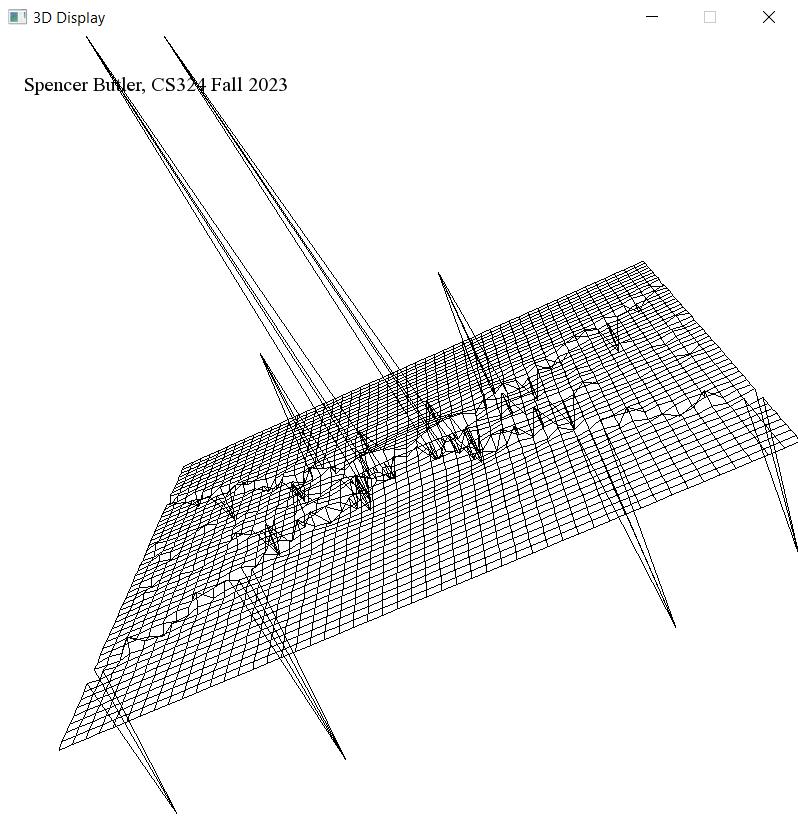
\includegraphics{img/0}
\subsection{Rubik's cube with no gaps:}
\noindent 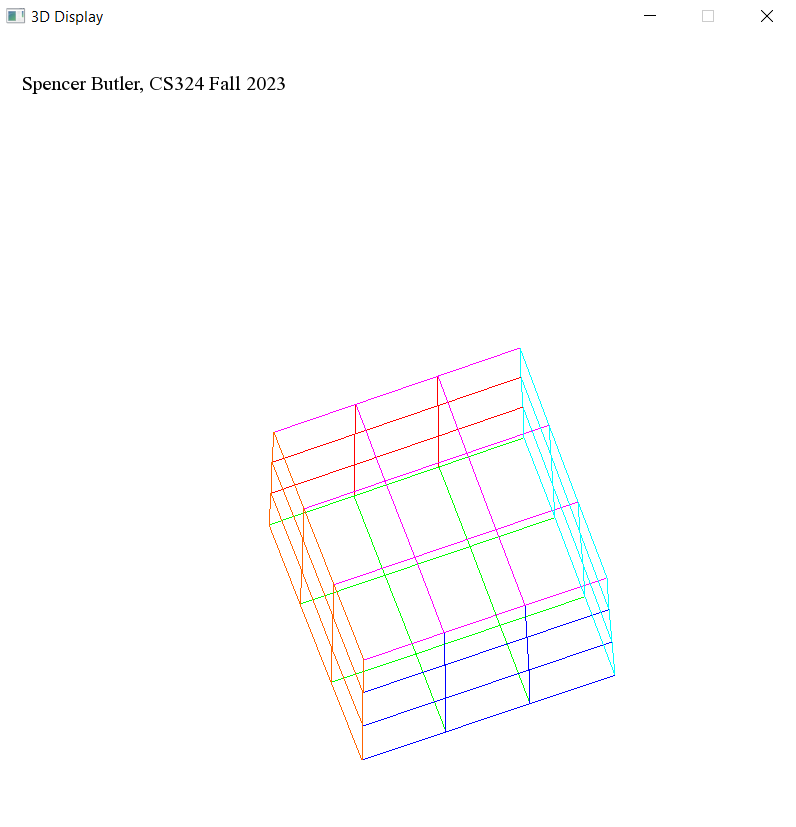
\includegraphics{img/1}
\subsection{Rubik's cube with gaps:}
\noindent 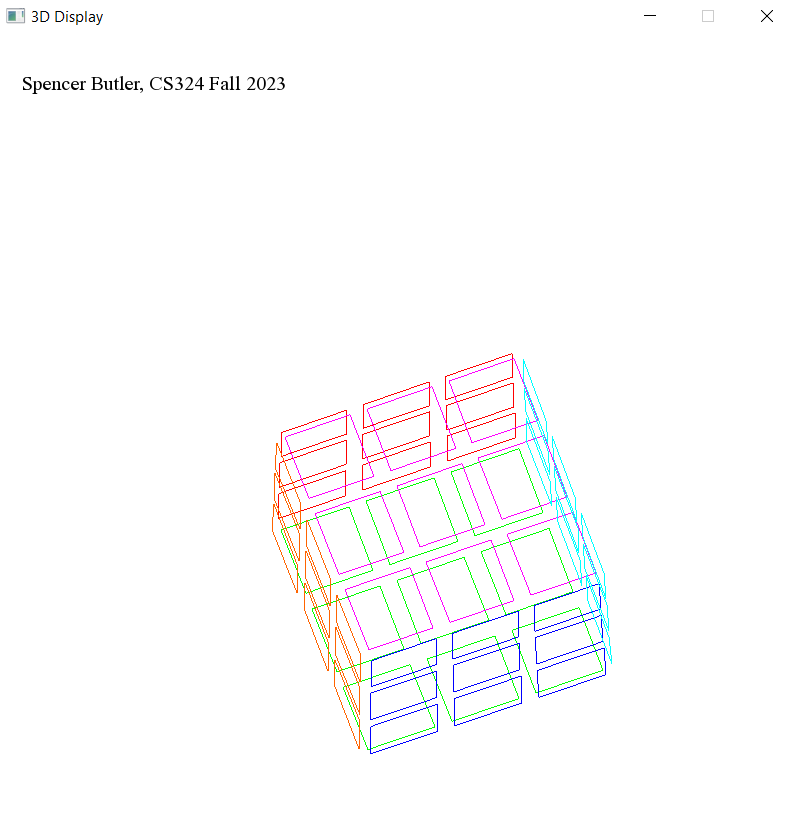
\includegraphics{img/2}
\subsection{Multiple Rubik's cubes with gaps:}
\noindent 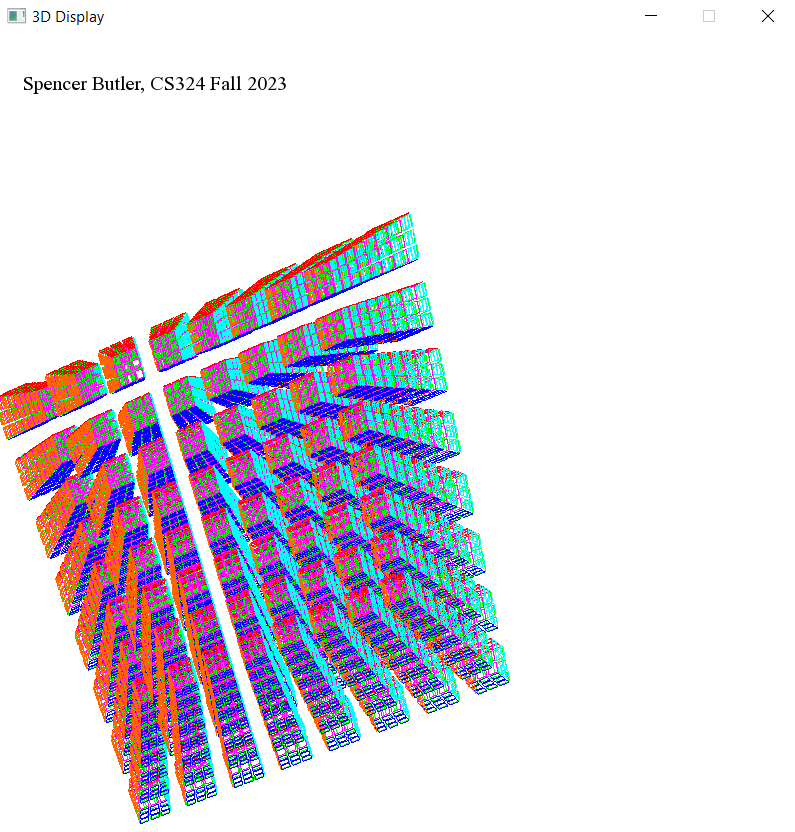
\includegraphics{img/3}
\subsection{Tron recognizer:}
\noindent 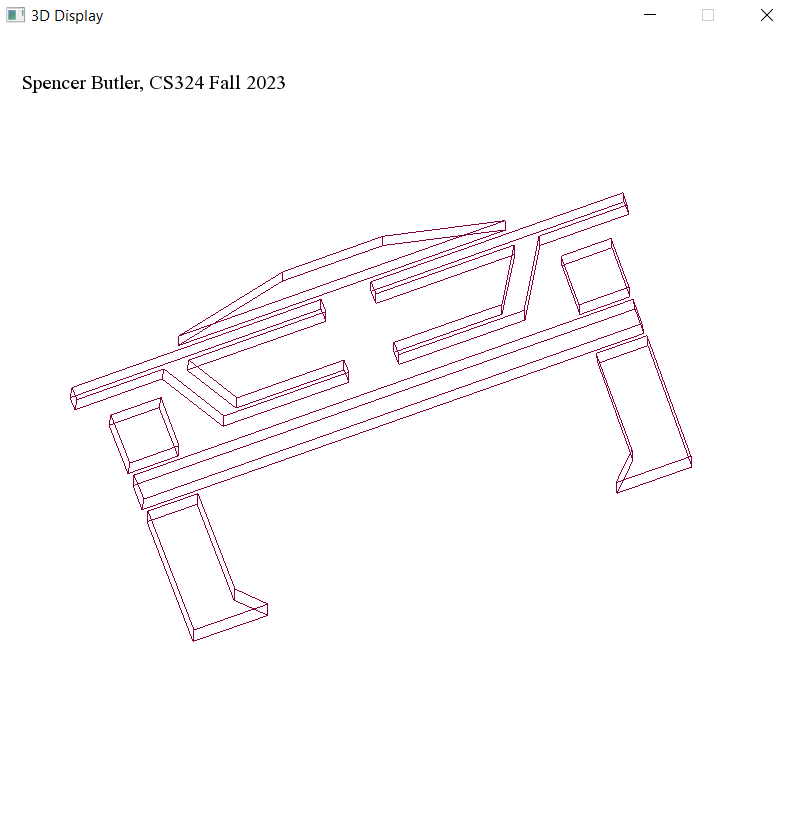
\includegraphics{img/4}
\subsection{My name in block letters:}
\noindent 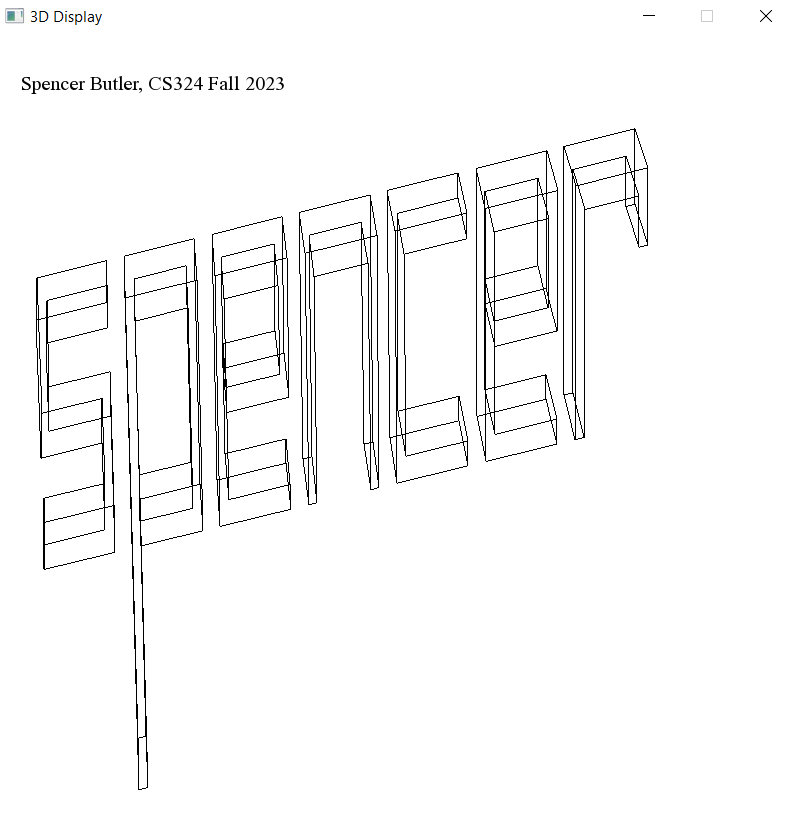
\includegraphics{img/5}


\end{document}

